\documentclass[spanish, a4paper, 11pt]{article}


\usepackage[T1]{fontenc}
\usepackage[utf8]{inputenc}

\usepackage{csquotes}
\usepackage{babel}

\usepackage[bookmarks=true]{hyperref}
\hypersetup{
	pdftitle={Reporte talle de integración},
	pdfauthor={Maximiliano Gaete, Josefa Miranda, Maria-Ignacia Rojas},
	pdfkeywords={},
	bookmarksnumbered,
	breaklinks=true,
	urlcolor=blue,
	citecolor=black,
	colorlinks=true,
	linkcolor=black,
}

\usepackage{lmodern}
\usepackage{amsmath}
\usepackage{amssymb}
\usepackage{textcomp}

\usepackage[style=ieee, citestyle=ieee]{biblatex}
\bibliography{references}

\usepackage{adjustbox}
\usepackage[
	per-mode=symbol,
	%output-decimal-marker={,},
	separate-uncertainty=true,
]{siunitx}

\usepackage{booktabs}
\usepackage{caption}
\captionsetup[table]{skip=1ex}

\usepackage{listings}
\lstset{basicstyle=\footnotesize\ttfamily,breaklines=true}
\usepackage{alltt}

\usepackage{tikz}
\usetikzlibrary{arrows.meta, positioning, shapes,arrows,calc}
\usepackage{graphicx}
\graphicspath{{figures/}}

\usepackage{pgfgantt}
\usepackage{placeins}

\usepackage{tikz}
\usepackage{cleveref}

\usepackage[
    % showframe,
	headheight=16mm,
    bottom=30mm,
]{geometry}

\usepackage{fancyhdr}
\setlength{\headheight}{80pt} % Ajustar a un valor más bajo si es posible
\addtolength{\topmargin}{-5pt} % Menos negativo si la cabecera ocupa mucho espacio
\fancypagestyle{unicamp}{
    \renewcommand{\headrulewidth}{0.4pt} 
    \renewcommand{\footrulewidth}{0pt}   
    
    \fancyhead{}
    \fancyfoot{}
    

    \fancyhead[L]{%
        \sffamily % Fuente sans-serif
        \begin{minipage}{0.3\textwidth}
            
\includegraphics[width=4cm]{./figures/logo.png}
        \end{minipage}%
        \begin{minipage}{0.7\textwidth}
            {\bfseries\fontsize{15.5pt}{1em}\selectfont\uppercase{Universidad de Valparaíso}}\\
            \fontsize{11.3pt}{1.2em}\selectfont\uppercase{Facultad de Ingeniería}\\
            \fontsize{11.3pt}{1.2em}\selectfont\uppercase{Escuela de Ingeniería Civil Biomédica}
        \end{minipage}
    }
    \fancyhead[R]{%
        \sffamily
        \vspace{2cm} 
    }
    
    \fancyfoot[C]{\sffamily\fontsize{9pt}{1em}\selectfont
        General Cruz 222 (ex-Edificio Hucke), Valparaíso, Chile\\
        \url{https://biomedica.uv.cl}}
}

\pagestyle{plain}

\usepackage{setspace}

\usepackage{relsize}
\usepackage{tikz}
\usetikzlibrary{arrows.meta, positioning}
\usepackage[nomain, acronym]{glossaries}
\setacronymstyle{long-sm-short}
\newcommand{\newacronymx}[8][]{%
	\newglossaryentry{#2}{
	type=\acronymtype,
	name={{\smaller #3}},
	sort={#3},
	first={#4 ({\smaller #3}, \emph{#5})},
	firstplural={#7 ({\smaller #6}, \emph{#8})},
	text={{\smaller #3}},
	plural={{\smaller #6}},
	description={#4 (\emph{#5})},#1}}

\newacronym{RTFM}{RTFM}{read the freaking manual}
\newacronymx{AOL}{AOL}{acronym in another language}{acrônimo em outra língua}{AOLs}{acronyms in another language}{acrônimos em outra língua}


\begin{document}

\thispagestyle{unicamp}

% Título 
\begin{center}

	\null\vfill

	{\scshape\large CBM 426 - Taller De integración\par}

	\vskip 3\baselineskip

	{\LARGE\bfseries Proyecto Incubadora\par}

	\vskip 3\baselineskip

	Alumnos:\\[1ex]
	{\large\bfseries Josefa Belen Miranda Aravena

	Maximiliano Antonio Gaete Pizarro

	Maria-Ignacia Rojas \par}

	\vskip 3\baselineskip

	Profesores:\\[1ex]
	{\large\bfseries Gonzalo Tapia Cabrera

	Antonio José Rienzo Renato

	Luis Togo Arredondo Gamboa\par}

\end{center}

\vfill


\newpage

\onehalfspacing

\tableofcontents

\newpage

\section{Introducción}

Se desarrollará un prototipo de incubadora neonatal que utiliza una ampolleta de 12V como fuente de calor, un ventilador para la circulación de aire, y un sensor NTC para medir la temperatura. 

La finalidad del prototipo y controlar de manera precisa la temperatura interna, creando un ambiente adecuado para un neonato. Para lograr esto, se implementará un sistema de control basado en Arduino que permite regular la temperatura de forma automática y eficiente. Además, se registrará la evolución de los parámetros obtenidos en diferentes escenarios, lo cual contribuye al análisis y mejora continua del prototipo.\par

\section{Objetivos}

\begin{enumerate}
    \item Desarrollar un prototipo de incubadora utilizando una caja plástica, con una ampolleta como calefactor, un ventilador y un sensor NTC para medir la temperatura.
    \item Diseñar un circuito controlado por Arduino que regule la potencia de la ampolleta, mida la velocidad del ventilador y registre la temperatura.
    \item Programar un software en Python que permita la comunicación del sistema con el computador a través de un puerto serial y controle los elementos mencionados.
    \item Realizar ensayos de control de temperatura y registrar los resultados en archivos CSV para su análisis posterior.
    \item Repetir los ensayos incluyendo el ventilador a distintas velocidades y generar gráficos de los resultados obtenidos.
    \item Desarrollar un modelo matemático que describa el comportamiento de la temperatura en función de la potencia del calefactor.
    \item Definir el rango de control de temperatura y los tiempos de respuesta del sistema.
    \item Implementar un algoritmo de control en Arduino para mantener la temperatura dentro del rango especificado.
    \item Verificar el funcionamiento del sistema y determinar el error máximo en la temperatura controlada.
    \item Crear una base de datos para registrar y visualizar el estado del prototipo en tiempo real.
    \item Implementar un sistema de alarmas luminoso y auditivo para alertar de fallos en el sistema.
    \item Registrar las alarmas del sistema dentro de la plataforma informática.
\end{enumerate}

\section{Diseño del Prototipo}

\subsection{Materiales}

\begin{table}[ht]
    \centering
    \caption{Materiales utilizados en el prototipo.}
    \begin{tabular}{ll}
        \toprule
        \textbf{Material} & \textbf{Cantidad} \\
        \midrule
        Caja plástica & 1 \\
        Ampolleta de 12V & 1 \\
        Ventilador de 12V & 1 \\
        NTC 100K & 1 \\
        Arduino Uno & 1 \\
        Protoboard & 1 \\
		Resistencia de 47\si{\ohm} & 1 \\
        Resistencia de 100\si{\ohm} 1W & 1 \\
        Resistencia de 5.6K\si{\ohm} & 1 \\
        Resistencia de 100K\si{\ohm} & 1 \\
        Transistor NPN 2N2222 & 1 \\
        Transistor NPN TIP41C & 1 \\
        Optoacoplador 4N26 & 1 \\
        Fuentes de alimentación 12V & 1 \\
        \bottomrule
    \end{tabular}
\end{table}
\FloatBarrier

\subsection{Dibujo Técnico}

\subsubsection{Tapa}

\begin{figure}[ht]
    \centering
    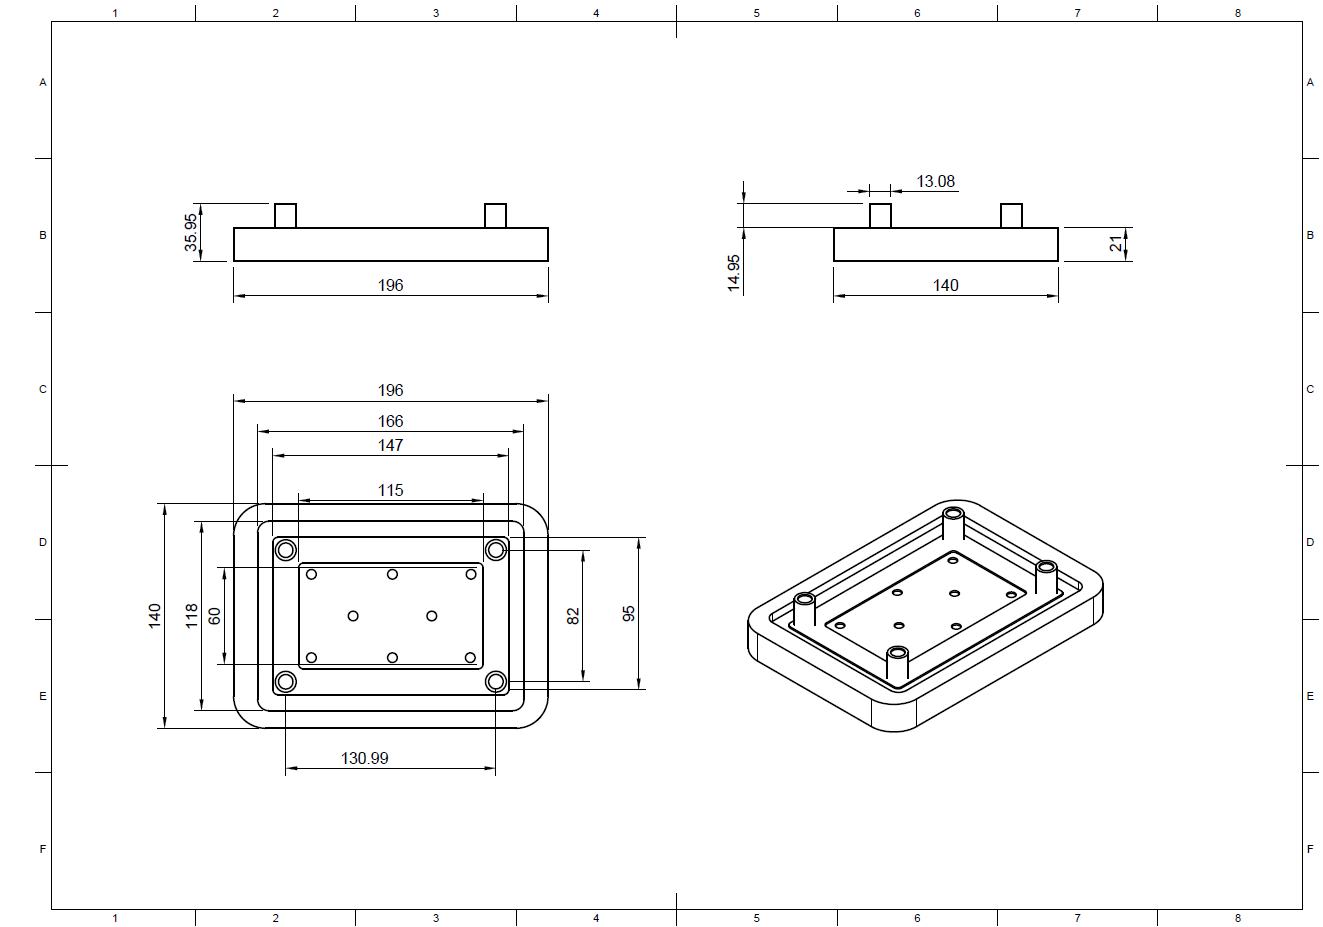
\includegraphics[width=0.75\textwidth]{./figures/Tapa.png}
    \caption{Dibujo técnico de la tapa.}   
\end{figure}
\FloatBarrier

\newpage
\subsubsection{Caja}

\begin{figure}[ht]
    \centering
    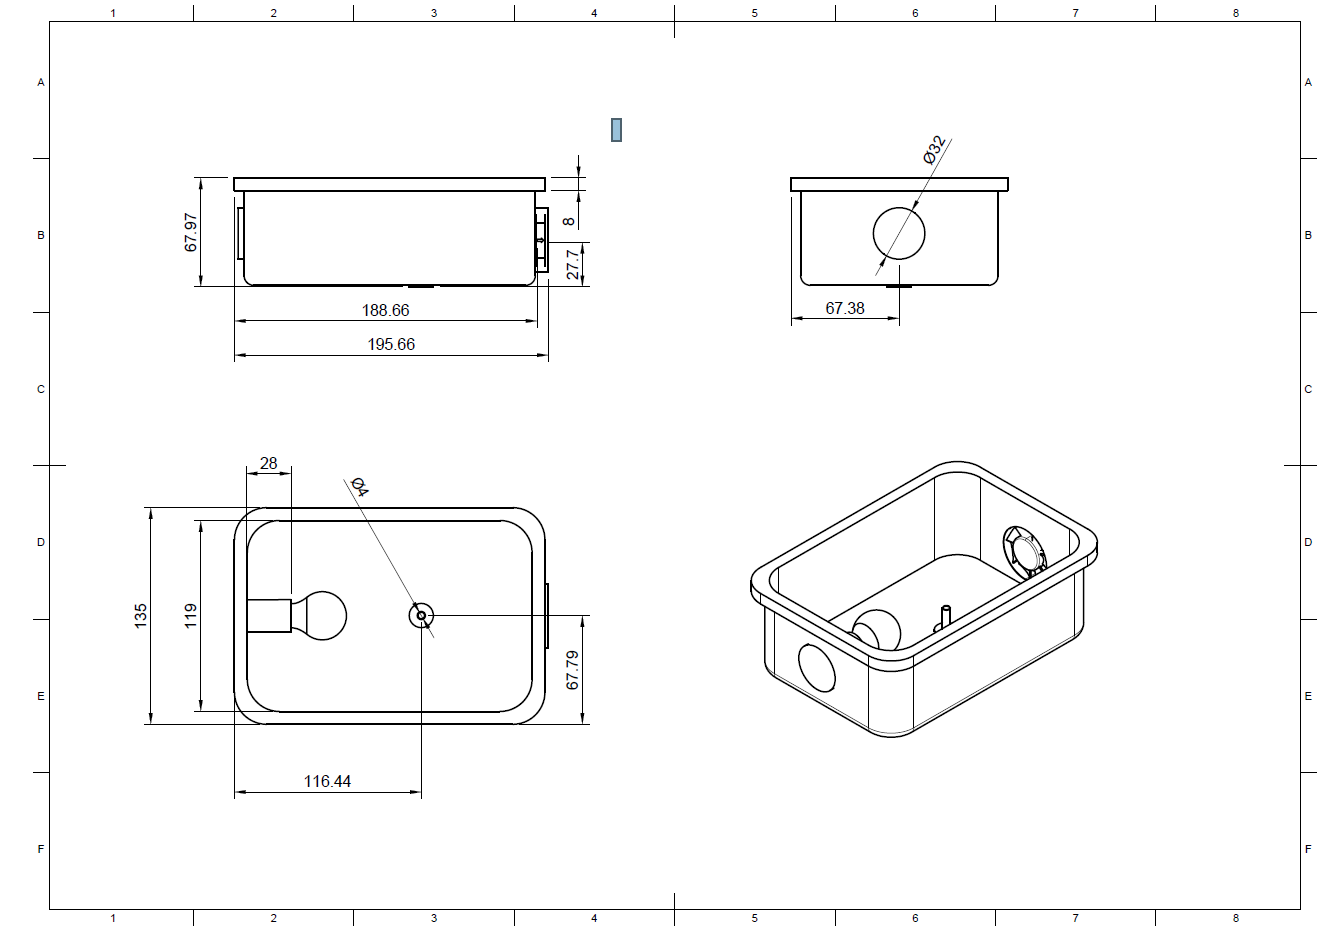
\includegraphics[width=0.7\textwidth]{./figures/Caja.png}
    \caption{Dibujo técnico de la caja plástica.}
\end{figure}
\FloatBarrier

\subsubsection{Caja Cerrada}

\begin{figure}[ht]
    \centering
    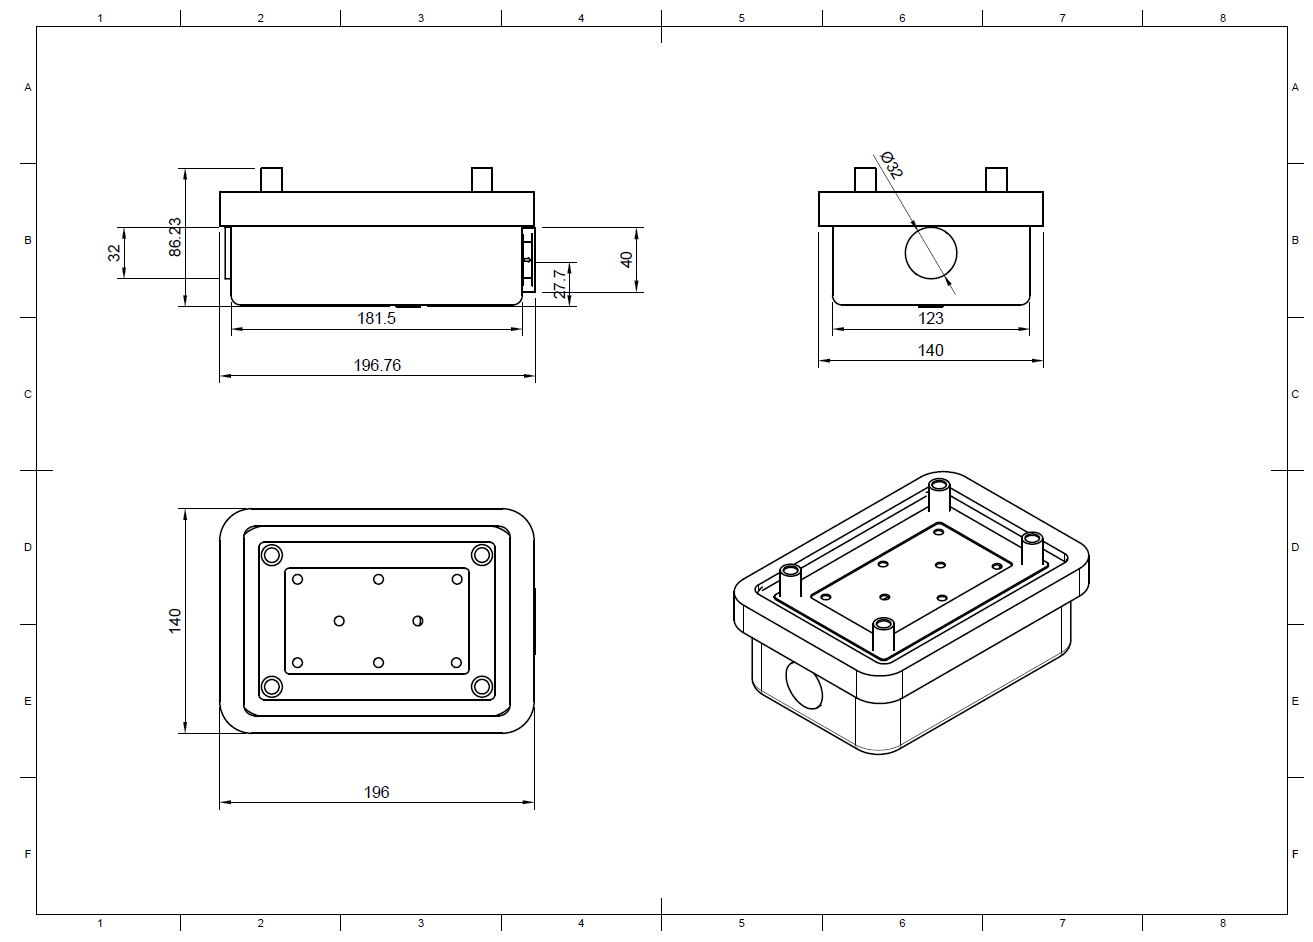
\includegraphics[width=0.7\textwidth]{./figures/Caja_completa.png}
    \caption{Dibujo técnico de la caja plástica con la tapa puesta.}
\end{figure}
\FloatBarrier

\subsection{Diseño del Circuito}

\subsubsection{Calculo de componentes a usar}

\subsubsection*{Ampolleta de 12V y 1.7A}

Se utilizará un transistor TIP41C para controlar la ampolleta, el cual tiene un rango de funcionamiento adecuado para la corriente que se manejará.

\[
i_A = 1.7 \, \text{A}
\]

El rango de \( h_{FE} \) para el transistor TIP41C es entre 15 y 75. En este caso, utilizamos un valor de \( h_{FE} \) mínimo:

\[
h_{FE} = 15
\]

La corriente de base \( i_b \) se calcula como:

\[
i_A = h_{FE} \cdot i_b
\]
\[
i_b = \frac{1.7}{15}
\]
\[
i_b = 0.113 \, \text{A}
\]

La resistencia de base \( R_b \) se calcula con la siguiente fórmula:

\[
R_b = \frac{12 - 0.7}{0.113}
\]
\[
R_b = 100 \, \Omega
\]

\subsubsection*{Ventilador de 12V y 0.06A}

Se utilizará un transistor 2N2222 para controlar el ventilador, el cual tiene un rango de funcionamiento adecuado para la corriente que se manejará.

\[
i_V = 0.06 \, \text{A}
\]

El rango de \( h_{FE} \) para el transistor 2N2222 es entre 30 y 75. Utilizaremos el valor mínimo de \( h_{FE} \):

\[
h_{FE} = 30
\]

La corriente de base \( i_b \) se calcula como:

\[
i_b = \frac{i_C}{h_{FE}}
\]
\[
i_b = \frac{0.06}{30} = 0.002 \, \text{A}
\]

La resistencia de base \( R_b \) se calcula de la siguiente manera:

\[
R_b = \frac{12 - 0.7}{0.002}
\]
\[
R_b = 5650 \, \Omega
\]

\subsubsection{Esquemático}

\begin{figure}[ht]
    \centering
    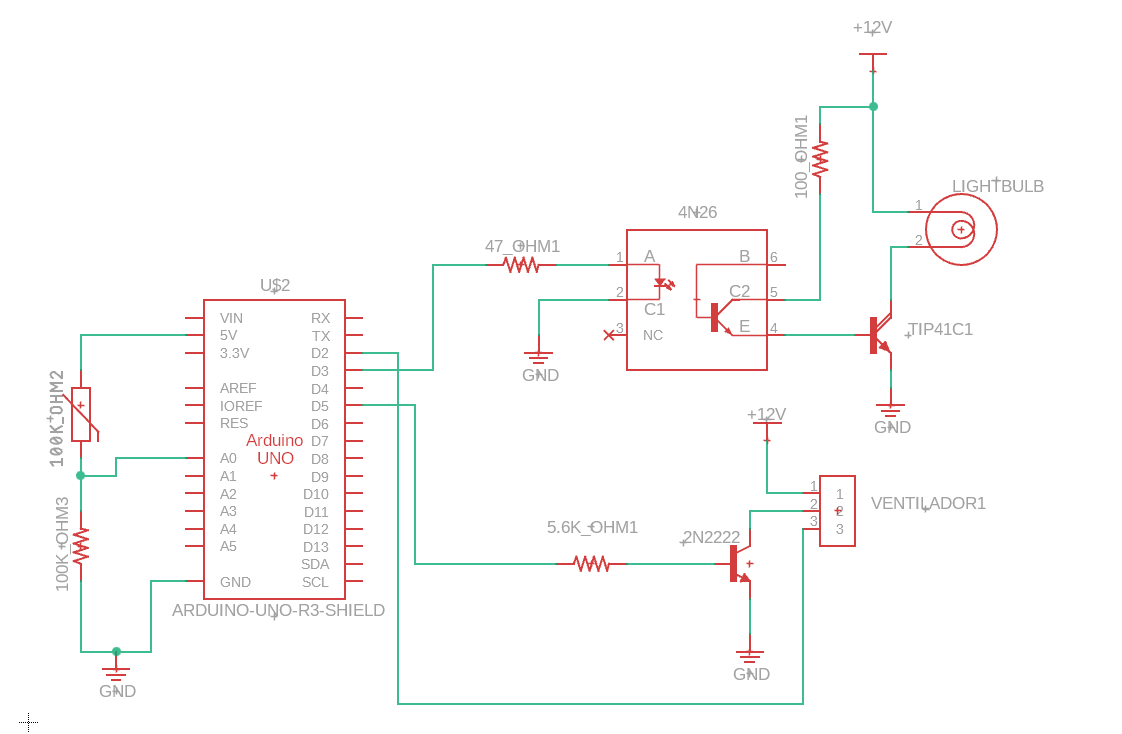
\includegraphics[width=0.7\textwidth]{./figures/Circuito.png}
    \caption{Diseño del circuito de control de la incubadora.}
\end{figure}
\FloatBarrier

\subsubsection{Circuito Impreso}

\begin{figure}[ht]
    \centering
    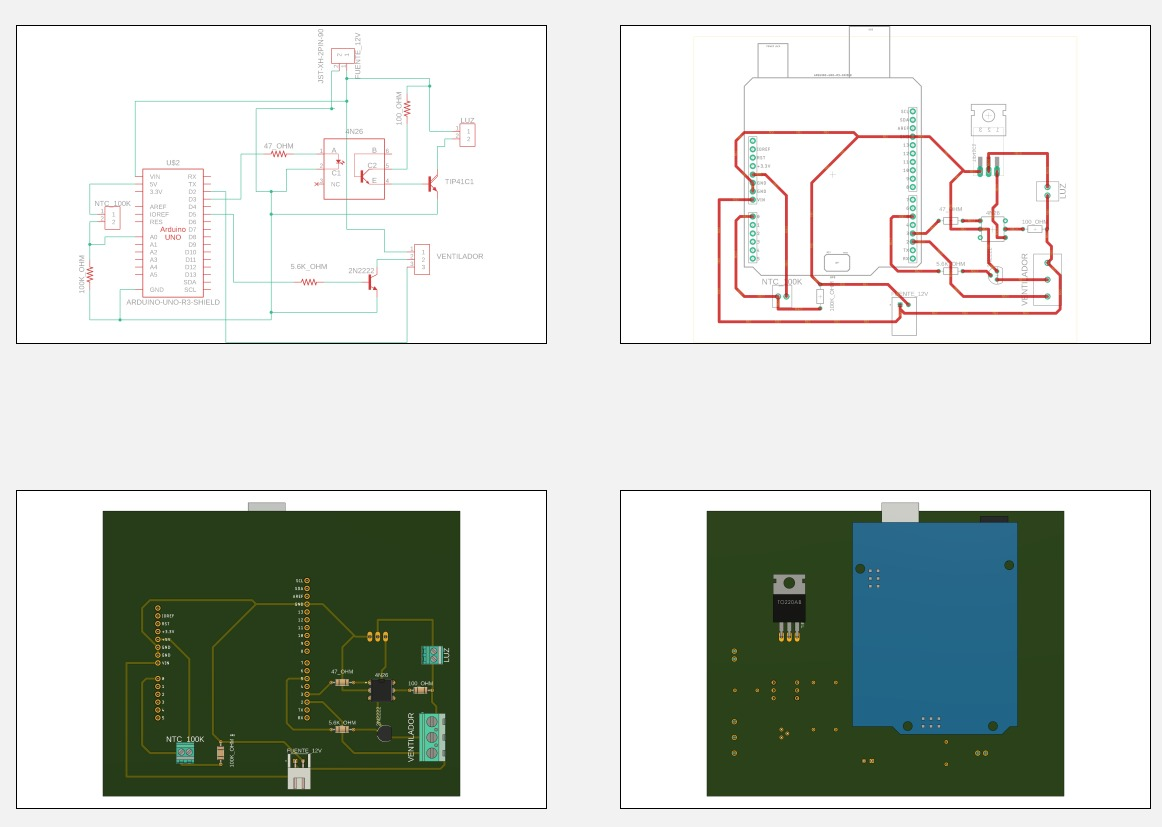
\includegraphics[width=0.6\textwidth]{./figures/PCB.png}
    \caption{Diseño del circuito impreso de control de la incubadora.}
\end{figure}
\FloatBarrier

\section{Código para el control de la incubadora}

Este proyecto integra dos componentes principales: un microcontrolador basado en Arduino y una interfaz gráfica desarrollada en Python utilizando la biblioteca PyQt6. El sistema permite controlar la potencia de radiación de una ampolleta, la velocidad de giro del ventilador, y medir la temperatura registrada por un sensor NTC. A continuación, se detallan los códigos implementados en ambas plataformas, explicando su funcionamiento.

\subsection{Código Arduino}

El código de Arduino es responsable de controlar los sensores y actuadores de la incubadora. Se utiliza un controlador PID (Proporcional, Integral y Derivativo) para mantener la temperatura estable, y se implementan las siguientes funciones:

\begin{itemize}
    \item {\bf Controlar la potencia de radiación de la ampolleta:} La ampolleta se controla utilizando modulación por ancho de pulso (PWM) en el pin 11 de Arduino. El valor de salida del controlador PID ajusta dinámicamente la potencia de la luz en función de la temperatura medida, o se puede ajustar manualmente desde la interfaz Python. Esto se logra con la función \texttt{analogWrite}.

    \item {\bf Controlar y medir la velocidad de giro del ventilador:} El ventilador se controla mediante PWM en el pin 9. La velocidad de giro se mide con un tacómetro conectado al pin 2, utilizando interrupciones para contar los impulsos por revolución. Estos valores se imprimen periódicamente por el puerto serial y se utilizan tanto para la visualización en la interfaz como para ajustar el ventilador.

    \item {\bf Medir la temperatura registrada por la NTC:} La resistencia del sensor NTC se mide en el pin A0, y se utiliza la ecuación de Steinhart-Hart para convertir la resistencia a una temperatura en grados Celsius. El valor de temperatura es utilizado por el PID para controlar la ampolleta.

\end{itemize}

A continuación se presenta el código de Arduino que implementa estas funciones:

\begin{lstlisting}[language=C++]
#include <Arduino.h>
#include <PID_v1.h>

// Definicion de pines y constantes
#define NTC_PIN A0
#define LUZ_PIN 11
#define VENT_PIN 9
#define VEL_PIN 2

// Coeficientes de la ecuacion de Steinhart-Hart para el sensor NTC
#define A_COEFF 0.5458630405e-3
#define B_COEFF 2.439180157e-4
#define C_COEFF -0.0003705076153e-7

// Variables para mediciones y control
float resistenciaNTC, logResistencia, tempKelvin, tempCelsius;
int lecturaNTC, potenciaVentilador, potenciaLuz;
volatile int contadorImpulsos = 0;
volatile float velocidadRPM = 0;
unsigned long tiempoAnteriorTemp, tiempoAnteriorVel, tiempoImprimir, ultimoTiempoRPM;

// Variables PID
double Setpoint, Input, Output;
double Kp = 30.0, Ki = 1.0, Kd = 0.0;
PID myPID(&Input, &Output, &Setpoint, Kp, Ki, Kd, DIRECT);

// Inicializacion de funciones y configuracion de pines
void setup() {
    Serial.begin(115200);
    pinMode(NTC_PIN, INPUT);
    pinMode(LUZ_PIN, OUTPUT);
    pinMode(VENT_PIN, OUTPUT);
    attachInterrupt(digitalPinToInterrupt(VEL_PIN), medirVelocidad, FALLING);
    myPID.SetMode(AUTOMATIC);
    myPID.SetOutputLimits(0, 100);
}

void loop() {
    // Logica de medicion de temperatura y control PID
    // Medicion de la NTC, calculo de temperatura y control de la ampolleta
    if (millis() - tiempoAnteriorTemp >= 250) {
        lecturaNTC = analogRead(NTC_PIN);
        resistenciaNTC = 100000.0 * ((1023.0 / lecturaNTC) - 1.0);
        logResistencia = log(resistenciaNTC);
        tempKelvin = 1.0 / (A_COEFF + B_COEFF * logResistencia + C_COEFF * pow(logResistencia, 3));
        tempCelsius = tempKelvin - 273.15;

        // Control de la luz
        Input = tempCelsius;
        myPID.Compute();
        analogWrite(LUZ_PIN, map(Output, 0, 100, 0, 255));

        tiempoAnteriorTemp = millis();
    }

    // Control y medicion de la velocidad del ventilador
    if (millis() - tiempoAnteriorVel >= 1000) {
        unsigned long tiempoActual = millis();
        unsigned long tiempoTranscurrido = tiempoActual - ultimoTiempoRPM;
        int pulsos = contadorImpulsos;
        contadorImpulsos = 0;
        if (tiempoTranscurrido > 0) {
            velocidadRPM = (pulsos / 2.0) * (60000.0 / tiempoTranscurrido);
        }
        ultimoTiempoRPM = tiempoActual;
        tiempoAnteriorVel = tiempoActual;
    }

    // Impresion de datos por serial
    if (millis() - tiempoImprimir >= 300) {
        Serial.print(tempCelsius);
        Serial.print(";");
        Serial.print(velocidadRPM);
        Serial.print(";");
        Serial.println(Output);
        tiempoImprimir = millis();
    }
}
\end{lstlisting}

Este código maneja la lectura de la temperatura y la velocidad del ventilador, ajustando la potencia de la luz en función del controlador PID.

\subsection{Código Python}

El código en Python implementa una interfaz gráfica que permite al usuario monitorear y controlar en tiempo real los valores de temperatura, velocidad del ventilador y la potencia de la luz. Las principales funciones son:

\begin{itemize}
    \item {\bf Controlar la potencia de la luz:} Desde la interfaz, el usuario puede ajustar manualmente la potencia de la luz usando un slider, o puede activar el modo automático que delega el control a Arduino. El control se realiza enviando comandos seriales que son interpretados por el Arduino.

    \item {\bf Controlar la velocidad del ventilador:} De forma similar, el usuario puede ajustar la velocidad del ventilador manualmente o permitir que el sistema controle automáticamente en función de la temperatura.

    \item {\bf Monitorear la temperatura:} La temperatura leída por el sensor NTC en Arduino se envía al programa Python, donde se muestra en la interfaz gráfica junto con gráficos en tiempo real que muestran las tendencias de temperatura, velocidad y potencia.
\end{itemize}

A continuación se presenta un extracto del código Python que implementa estas funciones:

\begin{lstlisting}[language=Python]
import serial
from PyQt6 import uic, QtWidgets
from PyQt6.QtCore import QTimer, QDateTime

class Plataforma(QMainWindow):
    def __init__(self):
        super().__init__()
        uic.loadUi("Plataforma.ui", self)
        self.serial_port = serial.Serial('COM12', 115200, timeout=1)
        self.timer = QTimer()
        self.timer.timeout.connect(self.leer_datos)
        self.timer.start(300)

    def leer_datos(self):
        while self.serial_port.in_waiting > 0:
            linea = self.serial_port.readline().decode('utf-8').strip()
            if linea:
                datos = linea.split(';')
                if len(datos) == 3:
                    temp = float(datos[0])
                    velocidad = float(datos[1])
                    potencia_luz_aplicada = float(datos[2])
                    # Mostrar datos en la GUI
                    self.label_temperatura.setText(f'Temperatura: {temp:.1f} C')
                    self.label_velocidad.setText(f'Velocidad: {int(velocidad)} RPM')
                    self.label_potencia_luz.setText(f'Potencia Luz: {potencia_luz_aplicada:.0f}%')

    def enviar_luz(self, valor):
        comando = f'LUZ {valor}\n'
        self.serial_port.write(comando.encode('utf-8'))

    def enviar_ventilador(self, valor):
        comando = f'VENT {valor}\n'
        self.serial_port.write(comando.encode('utf-8'))

    def enviar_setpoint(self, valor):
        comando = f'SETPOINT {valor}\n'
        self.serial_port.write(comando.encode('utf-8'))
\end{lstlisting}

Este código se encarga de la interacción entre el usuario y el sistema a través de una interfaz gráfica, mostrando la temperatura y la velocidad del ventilador, y permitiendo ajustar la potencia de la luz y la velocidad del ventilador. Los comandos enviados por el puerto serial son procesados por el Arduino para ajustar los actuadores correspondientes.

\subsubsection*{Gráficos en tiempo real}

El programa utiliza PyQtGraph para generar gráficos en tiempo real que muestran la evolución de la temperatura, la velocidad del ventilador y las potencias de los actuadores a lo largo del tiempo.

\begin{lstlisting}[language=Python]
def actualizar_graficos(self):
    self.curve_temp.setData(self.tiempos, self.temperaturas)
    self.curve_vel.setData(self.tiempos, self.velocidades)
    self.curve_potencia_vent.setData(self.tiempos, self.potencias_ventilador)
\end{lstlisting}

Estos gráficos permiten al usuario monitorear el desempeño de la incubadora de manera visual y en tiempo real, lo que facilita el control del sistema y la toma de decisiones.

\begin{figure}[ht]
    \centering
    \includegraphics[width=0.8\textwidth]{./figures/Interfaz.png}
    \caption{Interfaz gráfica de la plataforma de control de la incubadora.}
\end{figure}
\FloatBarrier



\section{Ensayos y Resultados}

\subsection{Ensayos de Control de Temperatura}

Para realizar los ensayos se realizaron 5 pruebas de respuesta tipo escalon, variando la potencia de la ampolleta de 0 a 100\% en incrementos de 20\%. Los resultados obtenidos se muestran a continuación.

\newpage
\subsubsection{Prueba 1: 100\% de potencia}

\begin{figure}[ht]
    \centering
    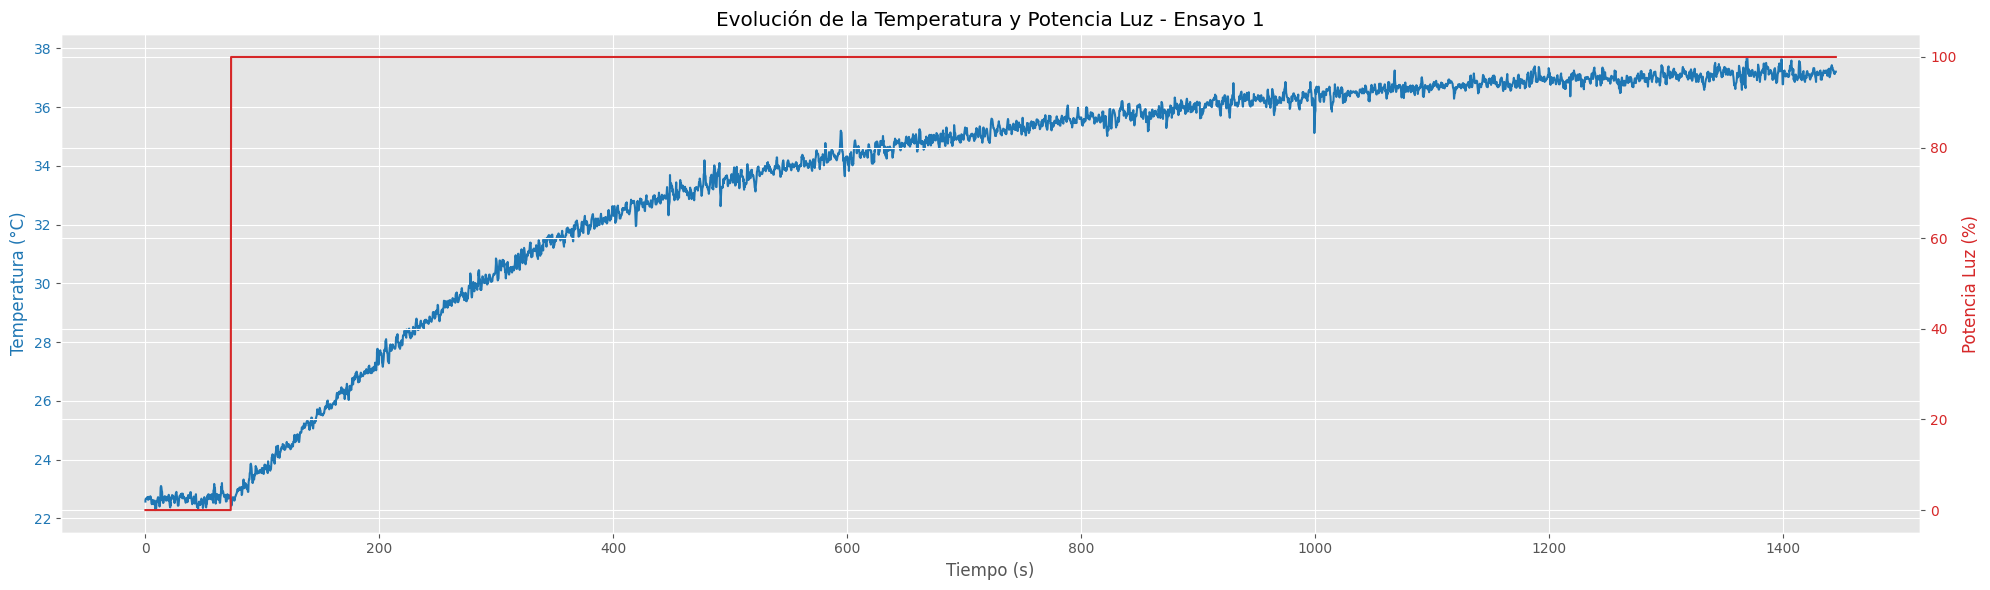
\includegraphics[width=0.9\textwidth]{./figures/prueba1.png}
    \caption{Respuesta de la temperatura a un escalón de 100\% de potencia.}
\end{figure}
\FloatBarrier

\subsubsection{Prueba 2: 80\% de potencia}

\begin{figure}[ht]
    \centering
    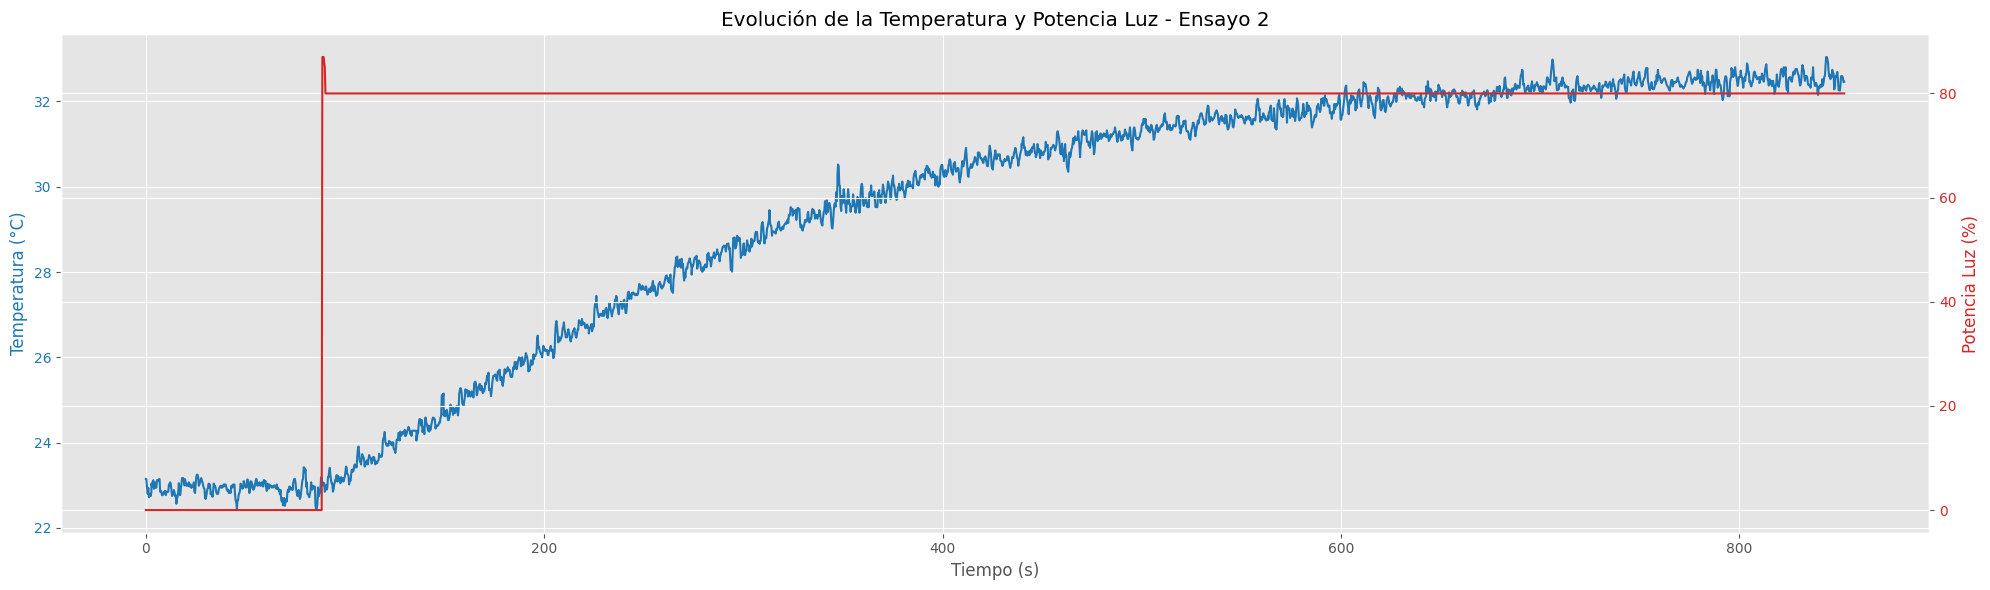
\includegraphics[width=0.9\textwidth]{./figures/prueba2.png}
    \caption{Respuesta de la temperatura a un escalón de 80\% de potencia.}
\end{figure}
\FloatBarrier

\subsubsection{Prueba 3: 60\% de potencia}

\begin{figure}[ht]
    \centering
    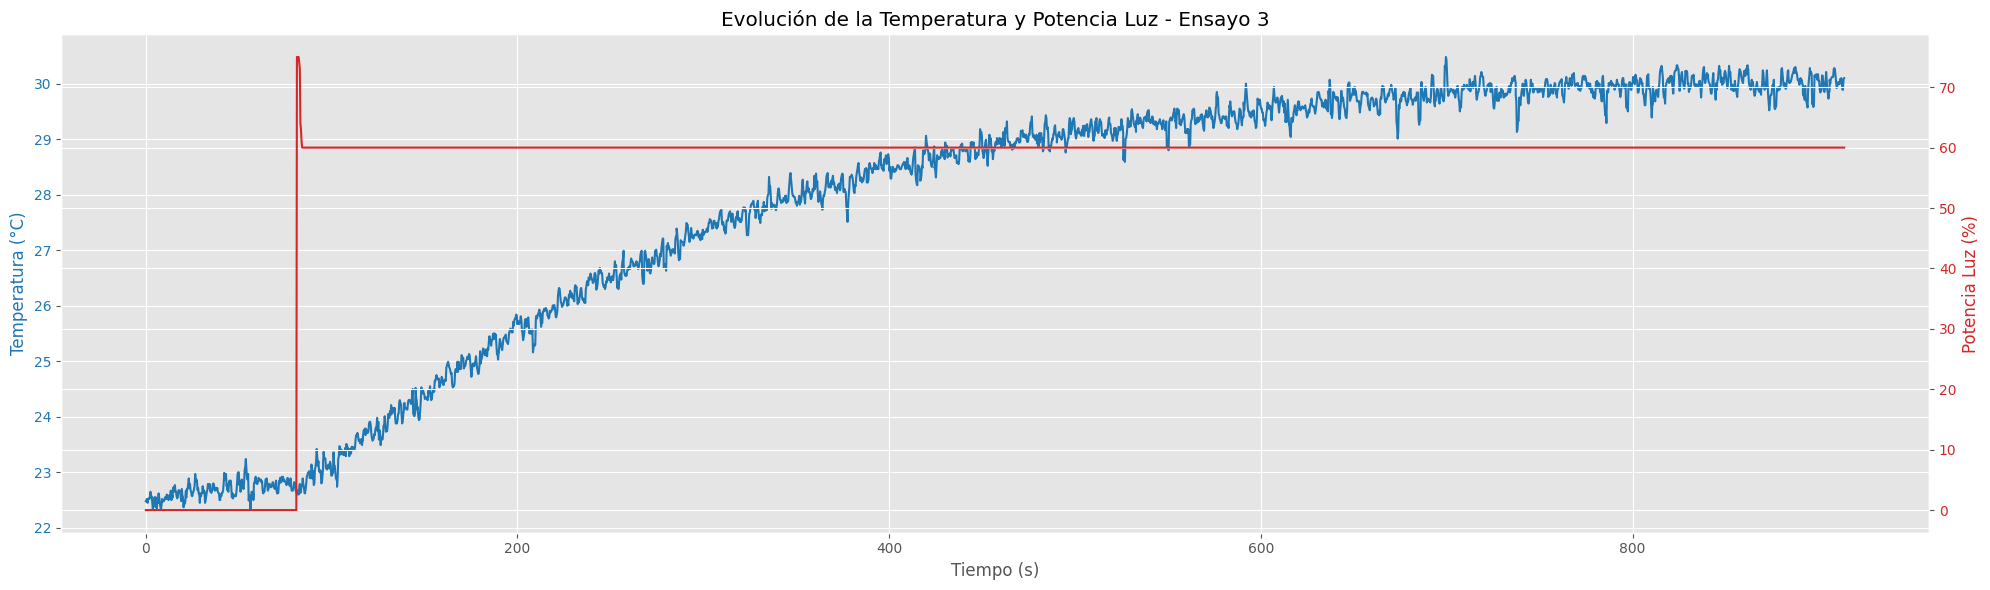
\includegraphics[width=0.9\textwidth]{./figures/prueba3.png}
    \caption{Respuesta de la temperatura a un escalón de 60\% de potencia.}
\end{figure}
\FloatBarrier

\newpage
\subsubsection{Prueba 4: 40\% de potencia}

\begin{figure}[ht]
    \centering
    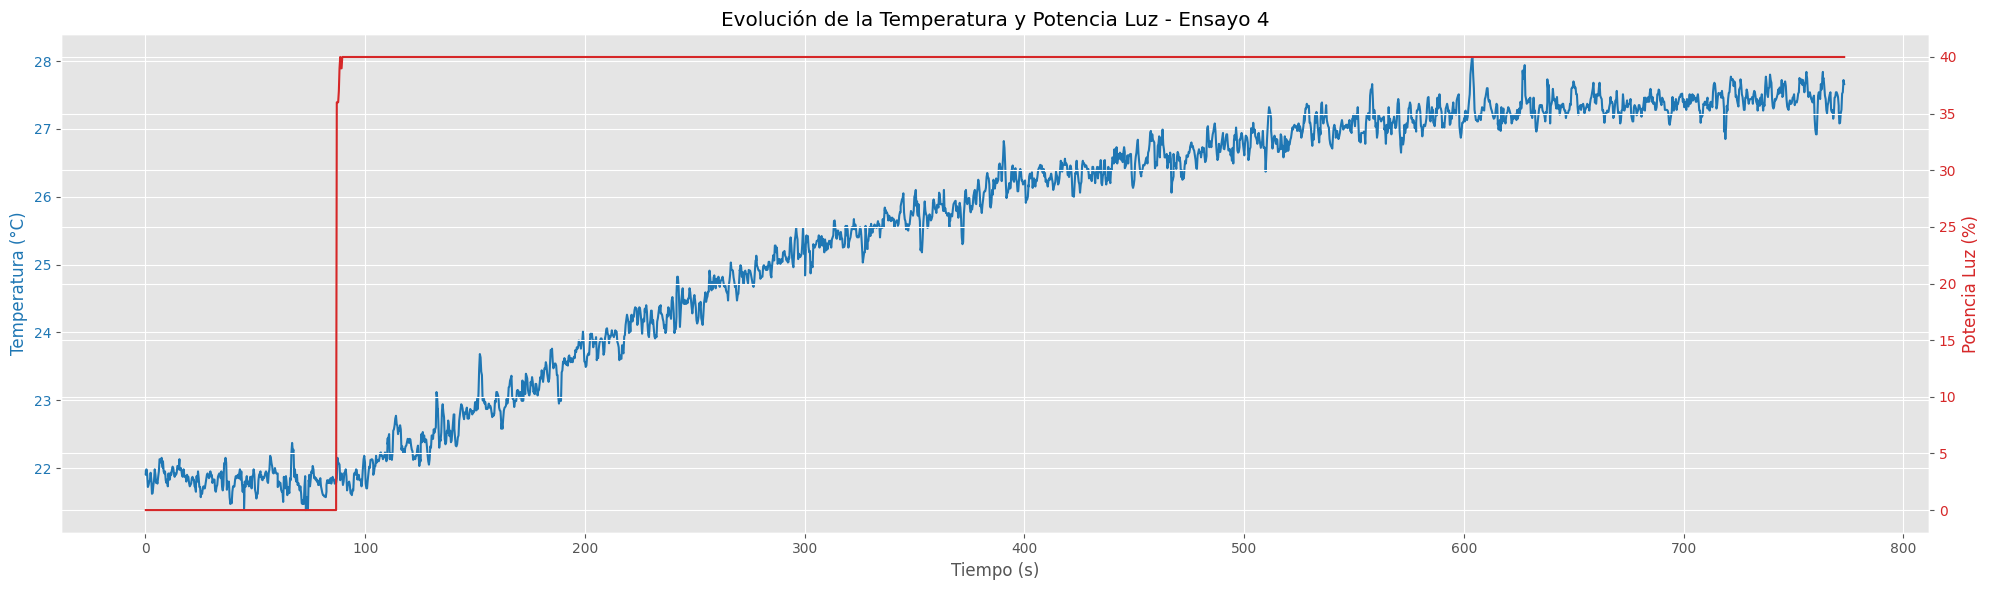
\includegraphics[width=0.9\textwidth]{./figures/prueba4.png}
    \caption{Respuesta de la temperatura a un escalón de 40\% de potencia.}
\end{figure}
\FloatBarrier

\subsubsection{Prueba 5: 20\% de potencia}

\begin{figure}[ht]
    \centering
    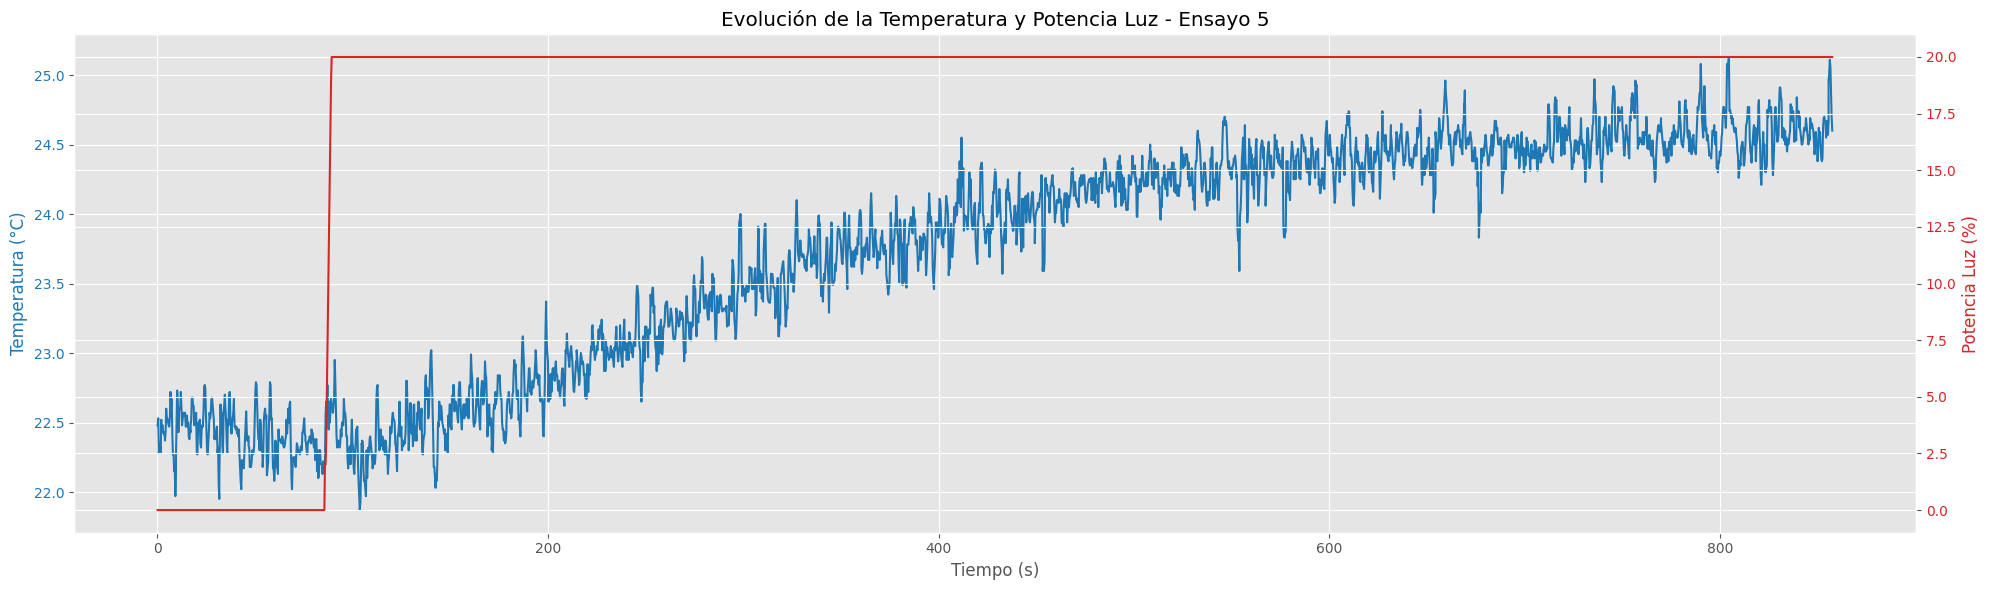
\includegraphics[width=0.9\textwidth]{./figures/prueba5.png}
    \caption{Respuesta de la temperatura a un escalón de 20\% de potencia.}
\end{figure}
\FloatBarrier

\subsection{Resultados de Respuesta Escalón de Temperatura}

Las pruebas de respuesta a escalón permiten evaluar la capacidad de control del sistema y determinar su desempeño en función de la potencia aplicada. La Potencia al 100\% representa la máxima capacidad de calentamiento de la ampolleta, mientras que la potencia al 0\% representa la condición de apagado total. 

Para realizar el análisis de los resultados, se calcula el tiempo de establecimiento \( t_s \), el sobrepaso máximo \( M_p \), la constante de tiempo \( K \), la temperatura maxima para cada ensayo.

\newpage

\section*{Fórmulas para el Analisis de la Respuesta a Escalón}

\subsubsection*{Cambio en la Temperatura Final (\( \Delta T_{\text{final}} \)):}
\[
\Delta T_{\text{final}} = T_{\text{final}} - T_{\text{inicial}}
\]

\subsubsection*{Ganancia Estática (\( K \)):}
\[
K = \frac{\Delta T_{\text{final}}}{\Delta P}
\]

\subsubsection*{Constante de Tiempo (\( \tau \)):}
\[
T_{\tau} = T_{\text{inicial}} + 0.632 \times \Delta T_{\text{final}}
\]

\subsubsection*{Tiempo de Asentamiento (\( t_s \)):}
\[
t_s \approx 4 \times \tau
\]

\subsubsection*{Sobrepaso (\( M_p \)) (si ocurre):}
\[
M_p = \frac{T_{\text{max}} - T_{\text{final}}}{T_{\text{final}}} \times 100
\]

\subsubsection{Cálculo de la Potencia de Radiación}

La potencia de radiación de la ampolleta se calcula como:

\[
P = V \cdot I
\]

Donde \( V = 12 \, \text{V} \) es el voltaje de la ampolleta y \( I \) es la corriente medida en cada ensayo.

En este caso la potencia total es de 20.4 W ya que los valores maximos alcanzados por la ampolleta son \( V = 12 \, \text{V} \) y \( I = 1.7 \, \text{A} \).

Al tener la eficiencia luminica de la ampolleta que es 0.05\%, se puede calcular la potencia de radiación.

\[
P_{\text{Radiación Luminica}} = P \cdot \text{Eficiencia}
\]

\[
P_{\text{Radiación calorica}} = P_{\text{Total}} - P_{\text{Radiación Luminica}}
\]
Esto se puede observar en el cuadro \ref{tab:escalones} para cada ensayo.

\begin{table}[ht]
    \resizebox{\textwidth}{!}{
    \begin{tabular}{|c|c|c|c|c|}
    \hline
    \textbf{Ensayo} & \textbf{Potencia (\%)} & \textbf{Potencia de Radiación. (W)}  \\ 
    \hline
    1 & 100 & 18.6  \\ 
    \hline
    2 & 80 & 14.9  \\ 
    \hline
    3 & 60 & 11.2  \\ 
    \hline
    4 & 40 & 7.4  \\ 
    \hline
    5 & 20 & 3.7 \\ 
    \hline
    \end{tabular}
    }
    \caption{Potencia de radiación según la potencia aplicada.\label{tab:escalones}}
\end{table}
\FloatBarrier

\subsubsection{Analisis Prueba 1: 100\% de potencia} 

\[
T_{\text{max}} = 37.43 \,^\circ\mathrm{C}
\]
\[
\Delta T_{\text{final}} = 37.13 - 23.25 = 13.88 \,^\circ\mathrm{C}
\]
\[
K = \frac{13.89}{100} = 0.1389 \,^\circ\mathrm{C/P\%}
\]
\[
t_s = 4 \times 296.12 = 1184.48 \, \text{s}
\]
\[
M_p = \frac{37.43 - 37.13}{37.13} \times 100 = 0.81\%
\]

\subsubsection{Analisis Prueba 2: 80\% de potencia}

\[
T_{\text{max}} = 32.69 \,^\circ\mathrm{C}
\]
\[
\Delta T_{\text{final}} = 32.52 - 22.95 = 9.57 \,^\circ\mathrm{C}
\]
\[
K = \frac{9.56}{80} = 0.1195 \,^\circ\mathrm{C/P\%}
\]
\[
t_s = 4 \times 236.68 = 946.72 \, \text{s}
\]
\[
M_p = \frac{32.69 - 32.52}{32.52} \times 100 = 0.52\%
\]

\subsubsection{Analisis Prueba 3: 60\% de potencia}

\[
T_{\text{max}} = 30.07 \,^\circ\mathrm{C}
\]
\[
\Delta T_{\text{final}} = 30.01 - 22.88 = 7.13 \,^\circ\mathrm{C}
\]
\[
K = \frac{7.13}{60} = 0.1188 \,^\circ\mathrm{C/P\%}
\]
\[
t_s = 4 \times 205.53 = 822.12 \, \text{s}
\]
\[
M_p = \frac{30.07 - 30.01}{30.01} \times 100 = 0.20\%
\]

\subsubsection{Analisis Prueba 4: 40\% de potencia}

\[
T_{\text{max}} = 27.72 \,^\circ\mathrm{C}
\]
\[
\Delta T_{\text{final}} = 27.46 - 21.79 = 5.67 \,^\circ\mathrm{C}
\]
\[
K = \frac{5.67}{40} = 0.1417 \,^\circ\mathrm{C/P\%}
\]
\[
t_s = 4 \times 216.53 = 866.12 \, \text{s}
\]
\[
M_p = \frac{27.72 - 27.46}{27.46} \times 100 = 0.95\%
\]

\subsubsection{Analisis Prueba 5: 20\% de potencia}

\[
T_{\text{max}} = 25.11 \,^\circ\mathrm{C}
\]
\[
\Delta T_{\text{final}} = 24.60 - 22.43 = 2.17 \,^\circ\mathrm{C}
\]
\[
K = \frac{2.17}{20} = 0.1085 \,^\circ\mathrm{C/P\%}
\]
\[
t_s = 4 \times 264.67 = 1058.68 \, \text{s}
\]
\[
M_p = \frac{25.11 - 24.60}{24.60} \times 100 = 2.07\%
\]

\subsubsection{Resultados Finales}
Para aclarar al lector, se presentan los resultados obtenidos en el cuadro \ref{tab:resultados}.

\begin{table}[ht]
    \resizebox{\textwidth}{!}{
    \begin{tabular}{|c|c|c|c|c|}
    \hline
    \textbf{Ensayo} & \textbf{Potencia (\%)} & \textbf{Temp. Inicial (°C)} & \textbf{Temp. Final (°C)} & \textbf{Cambio en Temp. (°C)} \\ 
    \hline
    1 & 100 & 23.25 & 37.13 & 13.88 \\ 
    \hline
    2 & 80 & 22.95 & 32.52 & 9.57 \\ 
    \hline
    3 & 60 & 22.88 & 30.01 & 7.13 \\ 
    \hline
    4 & 40 & 21.79 & 27.46 & 5.67 \\ 
    \hline
    5 & 20 & 22.43 & 24.60 & 2.17 \\ 
    \hline
    \end{tabular}
    }
    \caption{Resultados de los ensayos sin ventilador.\label{tab:resultados}}
\end{table}
\FloatBarrier

\subsection{Ensayos de Control de Velocidad del Ventilador}

Para realizar los ensayos se realizaron 5 pruebas de respuesta tipo escalon, variando la velocidad del ventilador. Los resultados obtenidos se muestran a continuación.

\subsubsection{Prueba 1: 100\% de Potencia, Ventilador a 12v, 9,5v y 7v}

\subsubsection{Prueba 2: 80\% de Potencia, Ventilador a 12v, 9,5v y 7v}

\subsubsection{Prueba 3: 60\% de Potencia, Ventilador a 12v, 9,5v y 7v}

\subsubsection{Prueba 4: 40\% de Potencia, Ventilador a 12v, 9,5v y 7v}

\subsubsection{Prueba 5: 20\% de Potencia, Ventilador a 12v, 9,5v y 7v}

\subsection{Resultados de Respuesta Escalón de Velocidad del Ventilador}

\subsubsection{Analisis Prueba 1: 100\% de Potencia, Ventilador a 12v, 9,5v y 7v}

\subsubsection{Analisis Prueba 2: 80\% de Potencia, Ventilador a 12v, 9,5v y 7v}

\subsubsection{Analisis Prueba 3: 60\% de Potencia, Ventilador a 12v, 9,5v y 7v}

\subsubsection{Analisis Prueba 4: 40\% de Potencia, Ventilador a 12v, 9,5v y 7v}

\subsubsection{Analisis Prueba 5: 20\% de Potencia, Ventilador a 12v, 9,5v y 7v}

\subsubsection{Resultados Finales}

Para aclarar al lector, se presentan los resultados obtenidos en el \ref{tab:resultados2}.

\begin{table}[ht]
    \resizebox{\textwidth}{!}{
    \renewcommand{\arraystretch}{1.5} % Ajusta el alto de las filas
    \setlength{\tabcolsep}{10pt}      % Ajusta el espacio horizontal entre columnas
    \begin{tabular}{|c|c|c|c|c|c|c|c|c|}
        \hline
        \textbf{Potencia (\%)} & \textbf{Ventilador (V)} & $T_{\text{inicial}}$ (°C) & $T_{\text{final}}$ (°C) & $\Delta T_{\text{final}}$ (°C) & $\tau$ (s) & $t_s$ (s) & $K$ (°C/P\%) & $M_p$ (\%) \\ 
        \hline
        100 & 7   & \dots & \dots & \dots & \dots & \dots & \dots & \dots \\ \hline
        100 & 9.5 & \dots & \dots & \dots & \dots & \dots & \dots & \dots \\ \hline
        100 & 12  & \dots & \dots & \dots & \dots & \dots & \dots & \dots \\ \hline
        80  & 7   & \dots & \dots & \dots & \dots & \dots & \dots & \dots \\ \hline
        80  & 9.5 & \dots & \dots & \dots & \dots & \dots & \dots & \dots \\ \hline
        80  & 12  & \dots & \dots & \dots & \dots & \dots & \dots & \dots \\ \hline
        60  & 7   & \dots & \dots & \dots & \dots & \dots & \dots & \dots \\ \hline
        60  & 9.5 & \dots & \dots & \dots & \dots & \dots & \dots & \dots \\ \hline
        60  & 12  & \dots & \dots & \dots & \dots & \dots & \dots & \dots \\ \hline
        40  & 7   & \dots & \dots & \dots & \dots & \dots & \dots & \dots \\ \hline
        40  & 9.5 & \dots & \dots & \dots & \dots & \dots & \dots & \dots \\ \hline
        40  & 12  & \dots & \dots & \dots & \dots & \dots & \dots & \dots \\ \hline
        20  & 7   & \dots & \dots & \dots & \dots & \dots & \dots & \dots \\ \hline
        20  & 9.5 & \dots & \dots & \dots & \dots & \dots & \dots & \dots \\ \hline
        20  & 12  & \dots & \dots & \dots & \dots & \dots & \dots & \dots \\ \hline
    \end{tabular}
    }
    \caption{Resultados de los ensayos con ventilador a diferentes velocidades y potencias.}
    \label{tab:resultados2}
\end{table}
\FloatBarrier
 
\newpage
\section{Modelo Matemático de la Incubadora de Control de Temperatura}  

Se presenta un modelo matemático para describir el comportamiento de la temperatura interna de un ambiente controlado como función de la potencia aplicada al calefactor. El modelo se basa en las suposiciones siguientes:

\begin{itemize}
    \item El efecto del ventilador se ignora.
    \item El sistema se aproxima como un sistema de primer orden.
    \item La temperatura inicial es \(T_0 = 22^\circ C\).
\end{itemize}

\subsection{Función de Transferencia}

Un sistema de primer orden en el dominio de Laplace se expresa mediante la siguiente función de transferencia:

\begin{equation}
    G(s) = \frac{K}{\tau s + 1}
\end{equation}

Donde:
\begin{itemize}
    \item \(G(s)\) es la función de transferencia del sistema.
    \item \(K\) es la ganancia estática promedio del sistema (\(0.1255 \, ^\circ C / P\%\)).
    \item \(\tau\) es la constante de tiempo promedio del sistema (243.91 s).
    \item \(s\) es la variable compleja del dominio de Laplace.
\end{itemize}

Sustituyendo los valores dados, obtenemos:

\begin{equation}
    G(s) = \frac{0.1255}{243.91 s + 1}
\end{equation}

\subsection{Ecuación Diferencial en el Dominio del Tiempo}

La ecuación diferencial equivalente en el dominio del tiempo es:

\begin{equation}
    243.91 \frac{dT(t)}{dt} + T(t) = 0.1255 \cdot P(t)
\end{equation}

\subsection{Solución en Estado Transitorio y Estacionario}

Para una entrada de potencia constante \(P(t) = P_0\), la solución es:

\begin{equation}
    T(t) = T_0 + K \cdot P_0 \cdot \left(1 - e^{-t/\tau}\right)
\end{equation}

En estado estacionario (\(t \to \infty\)), la temperatura alcanzada será:

\begin{equation}
    T_{\infty} = T_0 + K \cdot P_0
\end{equation}

Por ejemplo, si \(P_0 = 50\%\), la temperatura final será:

\begin{equation}
    T_{\infty} = 22 + 0.1255 \cdot 50 = 28.275 \, ^\circ C
\end{equation}

\subsection{Diagrama de Bloques}

A continuación se presenta el diagrama de bloques del sistema:

\begin{figure}[ht]
    \centering
    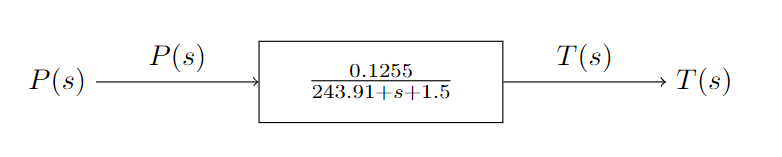
\includegraphics[width=1\textwidth]{./figures/DiagramaBloques.png}
    \caption{Diagrama de bloques del sistema de control de temperatura.}
\end{figure}
\FloatBarrier


\section{Temperaturas Alcanzables y Tiempo de Estabilización}

Para determinar el \textbf{rango de temperaturas alcanzable} mediante el control de la potencia del calefactor y los \textbf{tiempos de respuesta asociados}, nos basamos en la función de transferencia obtenida previamente:

\[
G(s) = \frac{0.1255}{243.91 \, s + 1}
\]

Donde:
\begin{itemize}
    \item $K = 0.1255$ °C/P\%: Ganancia estática del sistema.
    \item $\tau = 243.91$ s: Constante de tiempo.
    \item Temperatura inicial: $T_0 = 22$ °C.
\end{itemize}

\subsection{Rango de Temperaturas Alcanzable}

La temperatura máxima alcanzable dependerá de la potencia máxima aplicada al calefactor, que asumimos puede variar entre 0\% y 100\%. Usando la ganancia estática $K$, se calcula la temperatura final como:

\[
T_{\infty} = T_0 + K \cdot P_{\text{max}}
\]

Para $P_{\text{max}} = 100\%$:
\[
T_{\infty} = 22 + 0.1255 \cdot 100 = 34.55 \, \text{°C}
\]

Para $P_{\text{min}} = 0\%$:
\[
T_{\infty} = 22 + 0.1255 \cdot 0 = 22 \, \text{°C}
\]

Por lo tanto, el \textbf{rango de temperaturas alcanzable} es:

\[
22 \, \text{°C} \leq T \leq 34.55 \, \text{°C}
\]

\subsection{Tiempo de Respuesta del Sistema}

El tiempo de respuesta se refiere al tiempo que el sistema tarda en alcanzar un porcentaje significativo del valor final deseado. Para un sistema de primer orden, estos tiempos se calculan usando la constante de tiempo $\tau$.

\begin{itemize}
    \item \textbf{63.2\% del cambio total:}
    \[
    t_{63.2\%} \approx \tau = 243.91 \, \text{segundos} \approx 4.07 \, \text{minutos}
    \]

    \item \textbf{95\% del cambio total:} \\
    El tiempo para alcanzar el 95\% del valor final es aproximadamente 5 veces la constante de tiempo:
    \[
    t_{95\%} \approx 5 \cdot 243.91 = 1219.55 \, \text{segundos} \approx 20.33 \, \text{minutos}
    \]
\end{itemize}

\subsection{Resumen del Control de Temperatura}

\begin{itemize}
    \item \textbf{Rango de temperaturas alcanzable:}
    \begin{itemize}
        \item Mínima: 22 °C (sin potencia aplicada).
        \item Máxima: 34.55 °C (con 100\% de potencia).
    \end{itemize}
    \item \textbf{Tiempos de respuesta:}
    \begin{itemize}
        \item 63.2\% del valor final: $\approx 4.07$ minutos.
        \item 95\% del valor final: $\approx 20.33$ minutos.
    \end{itemize}
\end{itemize}

\subsection{Simulación en Python}

El siguiente código en Python simula la respuesta de la temperatura para diferentes niveles de potencia. La temperatura se calcula usando una función exponencial basada en el modelo de primer orden.

\begin{lstlisting}[language=Python]
import numpy as np
import matplotlib.pyplot as plt
import pandas as pd

# Simulacion de la Respuesta de Temperatura a Diferentes Potencias

% Parametros del sistema
K = 0.1268  % Ganancia estatica promedio (C/P%)
tau = 243.54  % Constante de tiempo promedio (s)
P_max = 100  % Potencia maxima (P%)

% Asumiendo que tienes un DataFrame con la columna 'Temperatura (C)'
df = pd.read_csv('tu_archivo.csv')  % Reemplaza con el nombre correcto del archivo
temperatura = df['Temperatura (C)']
T_inicial = temperatura[:50].mean()  % Temperatura inicial (C)

% Vector de tiempo para la simulacion
tiempo = np.arange(0, 1200, 1)  # Desde 0 hasta 1200 s en incrementos de 1 s

# Lista de niveles de potencia en porcentaje
niveles_potencia = [10, 20, 30, 40, 50, 60, 70, 80, 90, 100]

# Crear la figura para las graficas
plt.figure(figsize=(12, 8))

for porcentaje_potencia in niveles_potencia:
    # Calculo de P y T_final para cada nivel de potencia
    delta_P = P_max * (porcentaje_potencia / 100)
    delta_T_final = K * delta_P
    
    # Calculo de la temperatura en funcion del tiempo
    T = T_inicial + delta_T_final * (1 - np.exp(-tiempo / tau))
    
    # Graficar la respuesta
    plt.plot(tiempo, T, label=f'{porcentaje_potencia}% de Potencia')

# Configuracion de la grafica
plt.title('Simulacion de la Respuesta de Temperatura a Diferentes Potencias')
plt.xlabel('Tiempo (s)')
plt.ylabel('Temperatura (C)')
plt.legend()
plt.grid(True)
plt.show()
\end{lstlisting}

\subsection{Explicación del Código}

\begin{itemize}
    \item \textbf{Cálculo de $\Delta P$:} La potencia aplicada se calcula como un porcentaje de la potencia máxima.
    \item \textbf{Cálculo de $\Delta T_{\text{final}}$:} Se determina el aumento de temperatura esperado para cada nivel de potencia.
    \item \textbf{Simulación de la respuesta térmica:} La temperatura se calcula usando la ecuación:
    \[
    T(t) = T_{\text{inicial}} + \Delta T_{\text{final}} \cdot (1 - e^{-t/\tau})
    \]
    \item \textbf{Gráfica:} Se generan curvas de temperatura en función del tiempo para diferentes niveles de potencia.
\end{itemize}

\subsubsection*{Resultados Simulaciones}

El sistema permite controlar la temperatura interna entre \textbf{22 °C y 34.55 °C} según la potencia aplicada. El tiempo de respuesta para alcanzar el 95\% del valor final es de aproximadamente \textbf{20 minutos}. La simulación en Python confirma estos resultados mostrando cómo la temperatura evoluciona con diferentes niveles de potencia.

\begin{figure}[ht]
    \centering
    \includegraphics[width=1\textwidth]{Simulación de la Respuesta.png}
    \caption{Simulación de la Respuesta de Temperatura a Diferentes Potencias}
\end{figure}
\FloatBarrier

\section{Algoritmo de Control PID en Arduino} 


El sistema a controlar es de naturaleza térmica, lo que implica una respuesta lenta a los cambios. Dado que no se espera un comportamiento rápido o cambios bruscos, se ha decidido utilizar un \textbf{controlador PI} (Proporcional-Integral) en lugar de un PID completo. La ausencia del término derivativo evita amplificar el ruido proveniente del sensor de temperatura.

\subsection{Cálculo de los Parámetros del PID}

El controlador PID se define por tres constantes:
\begin{itemize}
    \item \textbf{Proporcional} ($K_p$): Controla la magnitud de la respuesta al error actual.
    \item \textbf{Integral} ($K_i$): Corrige errores acumulados en el tiempo, útil para eliminar el error en estado estacionario.
    \item \textbf{Derivativo} ($K_d$): Anticipa cambios futuros en el error, útil para sistemas rápidos. Sin embargo, no es necesario en sistemas térmicos.
\end{itemize}

Selección de los Valores:
\begin{itemize}
    \item $K_p = 30.0$: Un valor alto para corregir rápidamente los errores iniciales.
    \item $K_i = 1.0$: Un valor moderado para evitar acumulación excesiva del error, proporcionando estabilidad en el estado estacionario.
    \item $K_d = 0.0$: No se utiliza el término derivativo debido a la lentitud y ruido del sistema.
\end{itemize}

Estos valores fueron determinados empíricamente mediante prueba y error usando el metodo \textbf{Ziegler-Nichols}, ajustando los parámetros hasta lograr una respuesta rápida sin oscilaciones significativas.

\subsection{Implementación en Arduino}

\begin{lstlisting}[language=C++]
#include <PID_v1.h>

// Variables PID
double Setpoint, Input, Output;
double Kp = 30.0, Ki = 1.0, Kd = 0.0;
PID myPID(&Input, &Output, &Setpoint, Kp, Ki, Kd, DIRECT);

// Control automatico
bool control_automatico = false;
float ultimasTemp[5] = {0};
int indiceTemp = 0;


void setup() {
  Serial.begin(115200);

  // Configuracion del PID
  myPID.SetMode(AUTOMATIC);
  myPID.SetOutputLimits(0, 100);
}

void loop() {
  // Medicion de temperatura cada 250 ms
  if (millis() - tiempoAnteriorTemp >= 250) {
    lecturaNTC = analogRead(NTC_PIN);
    resistenciaNTC = 100000.0 * ((1023.0 / lecturaNTC) - 1.0);
    logResistencia = log(resistenciaNTC);
    tempKelvin = 1.0 / (A_COEFF + B_COEFF * logResistencia + C_COEFF * pow(logResistencia, 3));
    tempCelsius = tempKelvin - 273.15;

    ultimasTemp[indiceTemp] = tempCelsius;
    indiceTemp = (indiceTemp + 1) % 5;

    if (control_automatico) {
      Input = calcularPromedio(ultimasTemp, 5);
      myPID.Compute();
      analogWrite(LUZ_PIN, map(Output, 0, 100, 0, 255));
    }

    tiempoAnteriorTemp = millis();
  }

  // Envio de datos por Serial cada 300 ms
  if (millis() - tiempoImprimir >= 300) {
    Serial.print(calcularPromedio(ultimasTemp, 5));
    Serial.print(";");
    Serial.print(velocidadRPM);
    Serial.print(";");
    Serial.println(Output);
    tiempoImprimir = millis();
  }

  // Lectura de comandos desde Serial
  if (Serial.available() > 0) {
    String comando = Serial.readStringUntil('\n');

    if (comando == "AUTOMATIC_ON") control_automatico = true;
    else if (comando == "AUTOMATIC_OFF") control_automatico = false;
    else if (comando.startsWith("SETPOINT")) Setpoint = comando.substring(9).toDouble();
  }
}
\end{lstlisting}


Este diseño e implementación de un controlador PI en Arduino permite gestionar la temperatura del ambiente, la potencia de la luz sin cambios bruscos. Los valores PID fueron seleccionados empíricamente para obtener una respuesta rápida y estable. La exclusión del término derivativo es adecuada dado que se trata de un sistema lento con ruido en las mediciones. La estructura modular del código permite extenderlo fácilmente para otras funcionalidades ya que al separar el control manual del ventilador, ampolleta con el control automatico permite usar uno u otro cuando se requiera.

\subsection{Resultados Control de Temperatura con PID}


\section{Actividades y Cronograma}

Se adjuntan las Actividades realizas para el trabajo \cref{fig:gantt}.

\begin{figure}[ht]
	\centering
	\begin{ganttchart}[
			hgrid=true,
			vgrid=true,
			canvas/.append style={draw=none},
			title/.append style={draw=none},
			title label font=\small,
			bar label font=\small,
			y unit title=5mm,
			y unit chart=6mm,
			x unit=10mm,
		]{1}{6}
		\gantttitle{2015}{2}
		\gantttitle{2016}{4}\\
		\gantttitlelist{1,...,6}{1}\\
		\ganttbar{1.\ Bibliographical research}{1}{1}\\
		\ganttbar{2.\ Design}{2}{3}\\
		\ganttbar{3.\ Experiments}{3}{6}
	\end{ganttchart}
	\caption{Schedule of activities in trimesters.}
	\label{fig:gantt}
\end{figure}
\FloatBarrier

\section{Conclusion}

%\printbibliography

\end{document}